\title{A Reimplementation of Python’s dict using Simple Tabulation Hashing and Linear Probing}
\author{
        Russell Cohen \\
            \and
        Thomas Georgiou \\
            \and
        Pedram Razavi
}
\date{\today}
\documentclass[11pt]{article}
\usepackage[pdftex]{graphicx}
\usepackage{setspace}
\usepackage{fullpage}
\usepackage{float}


\begin{document}
\maketitle
\doublespace

\begin{abstract}
Here we implement simple tabulation hashing with linear probing in Python dictionary based on the recent theoretical result of Patrascu et al. Although we achieved small performance wins on the order of 4\%, we were unable to achieve significant performance wins.  The time and memory required to compute the ST hash are too large to justify the speedup garnered by switching to simple tabulation hashing and linear probing.
\end{abstract}


\section{Introduction}
In this project we aim to analyze and improve the performance of Python’s dictionary or dict.  Python is an extremely popular general purpose computing language for several reasons:
\begin{enumerate}
 \item Clean, elegant near-pseudo code syntax leads to clear code 
 \item Widely distributed and available
 \item Large quantity of external libraries for specific features 
\end{enumerate}

Recently, with the advent of packages like numPy, sciPy and pyPy Python has began to also be used (with questionable merit) as a performance computing language due to its ease of use.

However, because Python is an interpreted language it is difficult to operate on a similar performance level to compiled languages due to the sheer overhead of the interpreter.

In order to attempt to improve the performance of the python language as a whole we plan to attempt to improve the performance of python dictionaries.

\subsection{Motivation}
Python heavily utilizes dictionary data structure for several of its internal language features. This extensive internal use of dictionaries means that a running Python program has many dictionaries active simultaneously, even in cases where the the user’s program code does not explicitly use a dictionary. 

Take for example, the following code which we ran in the interpreter:

\begin{verbatim}
>> i = 2 
>> b = i * 2
>> b
10
\end{verbatim}

One of the features that we added to the python source was a conditional flag
that allowed us to view dictionary statistics (collisions, probes, accesses,
etc.) for a given invocation of the Python binary.  With that modification we
were able to see that this code used 92 lookups in string dictionaries and 24
lookups in general purpose dictionaries for a total of 116 dictionary hits. 116
hits in a 3 line piece of code which never uses dictionaries explicitly is quite
significant.  We explain this extensive dictionary usage below.

For instance, a dictionary can be instantiated to pass keyword arguments to a
function. This means a dictionary could potentially be created and destroyed on
every function call.  Some other examples of internal usage of dictionaries in
Python are as follows:

\begin{itemize}
\item Class method lookup
\item Instance attribute lookup and global variables lookup
\item Python built-ins module
\item Membership testing
\end{itemize}

Later in this paper, we compare the performance of our new dictionary
implementation for some of these special cases. The aforementioned applications
of the dictionaries further highlights the need for the fast instantiation and
deletion of dictionaries so that less memory is utilized once running a program.
Aside from the issue of memory usage, to further enhance the runtime of a
program we need fast key/value storage and retrievals which is the main focus of
this paper. Therefore it becomes clear that a better dictionary structure will
have significant effects on total Python performance.

\section{Current Python Implementation}

In this section we give a brief overview of the key implementation details of
dictionaries in CPython 2.7.3.  We should note that Python’s dictionary supports
several different data types as keys. However as we noted earlier, the
dictionaries underlying class instances and modules have only strings as keys.
Therefore optimizing a dictionary which have string-only keys is crucial to the
runtime of any Python program. CPython accommodates for this optimization by
changing its dictionary lookup method as necessary. First when a dictionary is
instantiated, CPython uses a string-only lookup function until a search for
non-string is requested, in this case CPython falls back to a more general
lookup method and uses this general function onward. There are two main
optimizations in the string-only lookup function.  First, since the string
comparisons do not raise any exceptions by design, some of the error checking
logic can been removed. Second, the string-only lookup function can skip the
rich set of comparisons ( $<=$, $>=$, $<$, $>$, $==$, $!=$) which arbitrary data
types can provide since string type does not have these special cases.  As it
can be seen, string-only keys can dominate the runtime of a dictionary and
CPython uses some measures to optimize for this common case. Because of this
importance we mostly limit ourselves to the study of new implementations of
hashing the string type for the rest of the paper.

The current CPython dictionary implementation uses an iterative XORed polynomial
terms for calculating the hash of the strings. In this implementation the hash
value for sequential strings differ only in the least significant bits, for
instance: hash("6.851") = 7824665118634166871 and hash("6.852") =
7824665118634166868. This behavior gives good results for sequential strings
which is a common case. When the table size is $2^i$ taking the least
significant $i$ bits as the index can populate the table without a lot of
collisions. This approach gives a better than random results in this case and is
also simple and fast to compute.

On the other hand this hashing strategy has the tendency to fill contiguous
slots of the hash table. CPython tries to solve this behavior by utilizing a
good collision resolution strategy. The collision resolution strategy currently
used is open addressing with a custom non-linear probing scheme. In this scheme
CPython uses quadratic probing based on this function: $j = (5j + 1) \bmod 2^i$
where $0<j<2^i-1$. This recurrence alone is not enough for a better behavior
since again it behaves the same as linear-probing for some keys since it scans
the table entries in a fixed order. To overcome this issue CPython also uses the
most significant bits of the hash value with the following code snippet:

\begin{verbatim}
slot = hash;
perturb = hash;
while (<slot is full> && <item in slot does not equal the key>) {
       slot = (5*slot) + 1 + perturb;
       perturb >>= 5;
}
\end{verbatim}

Based on this new method the probe sequence will depend on nearly all the bits
of a hash value. We should note that the value of  perturb shift (currently 5)
is crucial for a good probing behavior. Since it should be small enough so that
all the significant bits have an  effect on the probe sequence but at the same
time it should be large enough so that in really bad cases the high-order hash
bits can affect the earlier iterations.

CPython initializes its table with 8 slots. The resizing strategy is based on a
load factor invariant. Whenever there are $n$ keys in the dictionary, there must
be at least $3n/2$ slots in the table. This load factor is to keep the table
sparse and put a bound on the number of collisions that can happen. CPython
resizes the size of table whenever the load factor invariant gets violated. It
quadruples the size when there are less than 50,000 keys in the table and
doubles the size otherwise. 

Overall, the design of CPython dictionary is simple and is optimized for more
common cases such as sequential strings. Since it utilizes quadratic probing
with perturbation, even if a data type does not provide a good hash function,
the table still gets populated with with short chain lengths.  On the other hand
there are some behaviors which can be improved. For instance there is a bad
cache locality because for probing a slot the table might need to jump to the
other slots which are not immediate neighbors and not necessarily in cache. 

\section{Improvements}

\subsection{Theoretical Results}
Recently, Patrascu et al. [2] showed that simple tabulation hashing provides unexpectedly strong guarantees and is constant competitive with a truly random hash function for hashing with linear probing. They also showed some experimental evaluations which proved that simple tabulation on fixed input length can be fast and robust when used with linear probing and cuckoo hashing. 

Linear probing is appealing because of its excellent cache behavior in comparison to the probing scheme currently utilized in Python.  Consider the Intel Core 2 Duo processor with a 64 byte cache line.  Each Python dictionary entry is 12 bytes so when Python’s current probing scheme probes another slot, it is not in the current cache line so it has to pull another cache line in from memory, but with linear probing, that next slot is most likely in the current cache line.

However, Patrascu et al. [2] describe simple tabulation hashing for fixed key widths.  We will need to figure out a variant of simple tabulation hashing for variable length strings that does not require a table for every possible index (we could potentially cycle through a fixed set of tables).  Performing table lookups is potentially an expensive operation with lots of cache hits mitigating the better cache behavior of linear probing so we will have to be careful about how we implement it.

\subsection{Implementation Details}
We prepopulated random tables in memory with random bits from random.org, which sources randomness form atmospheric noise.
       
       \begin{verbatim}
    while (--len >= 0) {
        register long index = (*p++) | ((len&TABLE_MASK)<<8);
        x = x ^ RAND_TABLE_NAME[index];
    }
       \end{verbatim}

\subsubsection{Optimizations}

After implementation and profiling, we found that dictionary table lookups had
over twice as many level 1 cache misses with tabulation hashing than without.
Hypothesizing that the tabulation tables were evicting other, more relavant
data from the level 1 cache.  To fix this, we inserted x86 memory prefetch
instructions into our hash code to tell the CPU's caching system that it should
deprioritize storing it in cache.  We used GCC's
\begin{tt}\_\_builtin\_prefetch(void \*addr, char rw, char locality)\end{tt}
to do this.  However, this only yielded about a 1\% performance improvement.

\section{Results}

\subsection{Table Number Tuning}
       
We attempted to measure the 
See Figure ~\ref{fig:tables}
 \begin{figure}[H]
   \centering
   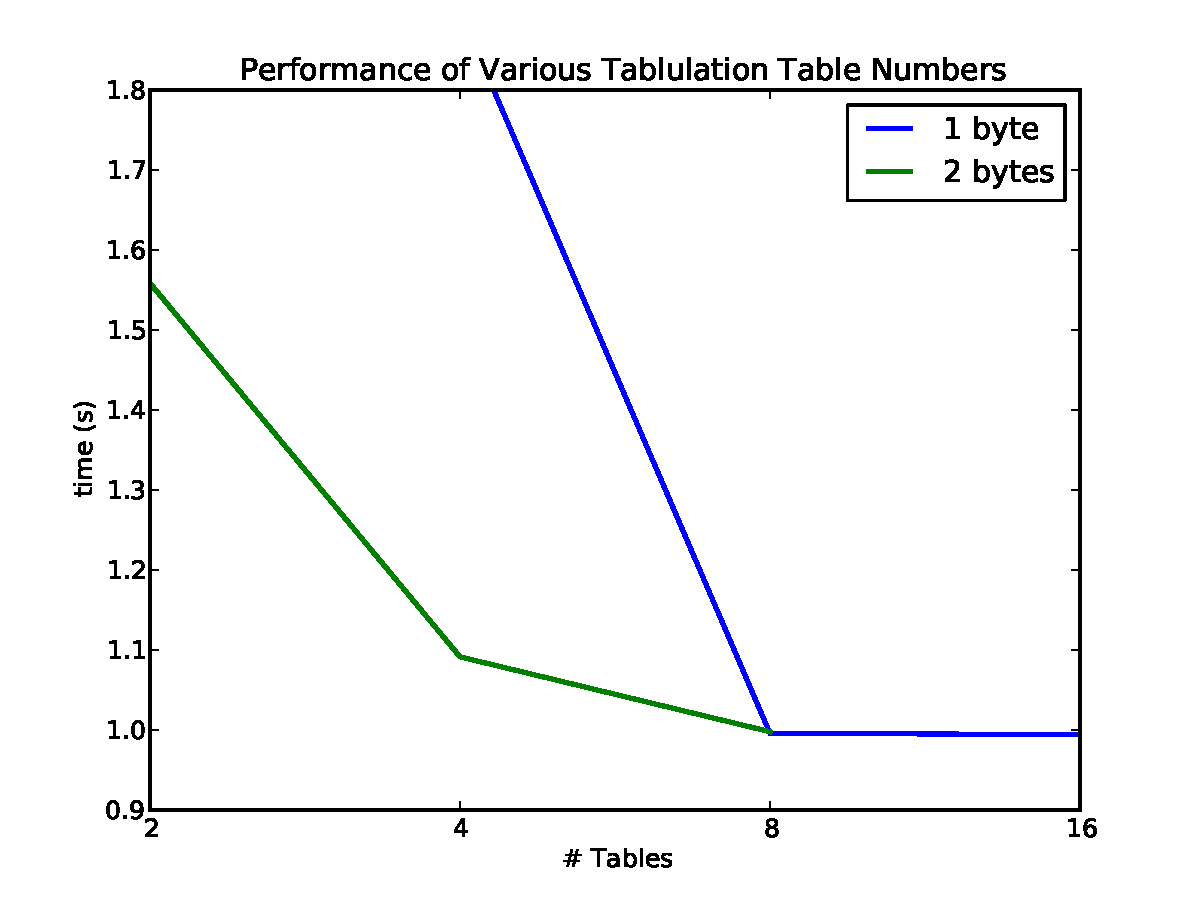
\includegraphics[width=4in]{tables.pdf}
   \caption{}
   \label{fig:tables}
 \end{figure}
       
Eight tables provided the best performance.
\subsection{Benchmarks}
In order to analyze the result of this new dictionary we measured three main metrics. First, we compared the performance of the simple tabulation hashing with Python’s current hashing scheme on random strings. Second, we measured the number of probes and collisions and overall the quality of our dictionary on structured and unstructured inputs. Finally, in this section  we show some of the total time spent in dictionary operations by using a set of general Python benchmarks and some real-world programs.
Because of the heavy utilization of dictionaries in Python internals one of the valuable benchmarks is to see how the new dictionary performs on them. We used PyBench benchmark suit for this task. We saw significant improvements of around \%20 in performance of some of the internals such as the special and normal class attribute lookups and string predicates. However, at the same time some of the other internals such as CPython exception handler were running around \%12 slower compared to the current implementation. On average a \%4.5 improvement in runtime was measures for running the whole benchmark suite.

\begin{table}
  \caption{Performance results on selected components of the PyBench suite.  We
    have ommitted the least significant performace results in terms of percent
    change.
  }
\begin{tabular}{| l | c |}
  \hline
  \textbf{Test Name} & \textbf{Performance Difference} \\ \hline
  Test Name & Performance Difference \\ \hline
  NormalClassAttribute &  19.20\% \\ \hline
  SpecialClassAttribute &  18.88\% \\ \hline
  NormalInstanceAttribute &  17.77\% \\ \hline
  StringPredicates &  15.25\% \\ \hline
  UnicodePredicates &  13.82\% \\ \hline
  SimpleListManipulation &  13.03\% \\ \hline
  CompareUnicode &  11.27\% \\ \hline
  SimpleComplexArithmetic &  10.83\% \\ \hline
  SpecialInstanceAttribute &  10.52\% \\ \hline
  TryFinally &  10.35\% \\ \hline
  CreateUnicodeWithConcat &  8.52\% \\ \hline
  StringSlicing &  6.52\% \\ \hline
  Small Performance Changes Ommitted & ... \\ \hline
  UnicodeMappings &  -1.27\% \\ \hline
  ListSlicing &  -2.40\% \\ \hline
  ComplexPythonFunctionCalls &  -3.55\% \\ \hline
  TupleSlicing &  -3.72\% \\ \hline
  WithRaiseExcept &  -5.89\% \\ \hline
  TryRaiseExcept &  -11.99\% \\ \hline
  Totals & 4.54\% \\ \hline
\end{tabular}
\end{table}

PyBench showed the performance difference in each of the individual CPython internals however for a more realistic picture of the performance in real world programs more extensive benchmarking of the new implementation was needed. Especially since we wanted to know the frequency of the different CPython internals in real-world applications and therefore the corresponding runtime changes. The new implementation was tested on several standard real world programs such as Tornado web server, Django web framework, html5lib and nearly 10 other real-world programs. 

We were interested to calculate if the new implementation of dictionary can handle more requests in a Python web server compared to the current CPython implementation. We chose Tornado web server for this task since most of the code is written in pure Python. An instance of Tornado server was run in a virtual machine with one assigned processor. The following code[http://nichol.as/benchmark-of-python-web-servers] was used as a sample Tornado application:
 \begin{verbatim}
import tornado.httpserver
import tornado.ioloop
import tornado.wsgi

def application(environ, start_response):
    status = '200 OK'
    output = 'Pong!' 
    response_headers = [('Content-type', 'text/plain'),
        ('Content-Length', str(len(output)))]
    start_response(status, response_headers)
    return [output]
def main():
    container = tornado.wsgi.WSGIContainer(application)
    http_server = tornado.httpserver.HTTPServer(container)
    http_server.listen(8000)
    tornado.ioloop.IOLoop.instance().start()
if __name__ == "__main__":
    main()
 \end{verbatim}

Different request rates (up to 2000 requests per second) were tested on this sample server and their corresponding response rates were calculated using httpef, a HTTP performance measurement tool. Considering the variance of request rates on different iterations of the test, we could not find any significant improvement of the response rate of the new implementation. We found that on the average performance was similar however the new implementation showed a smaller standard deviation in the response rates. This finding followed by other benchmarks showed that the new implementation gives more consistent runtime on different iterations of a same code compared to the current CPython implementation. This consistency is a desired behavior. We suspect that this behavior is a result of the randomness of hash values in simple tabulation hashing and also the smaller average chain lengths.

As mentioned before, another set of the benchmarks that we utilized were based on different standard real-world Python applications. We ran and timed the performance of the new implementation and CPython 2.7.3 side by side using the Python-Mirrors suite. The performance of more than ten applications were recoded as shown in the figures.

\begin{figure}[H]
  \centering
  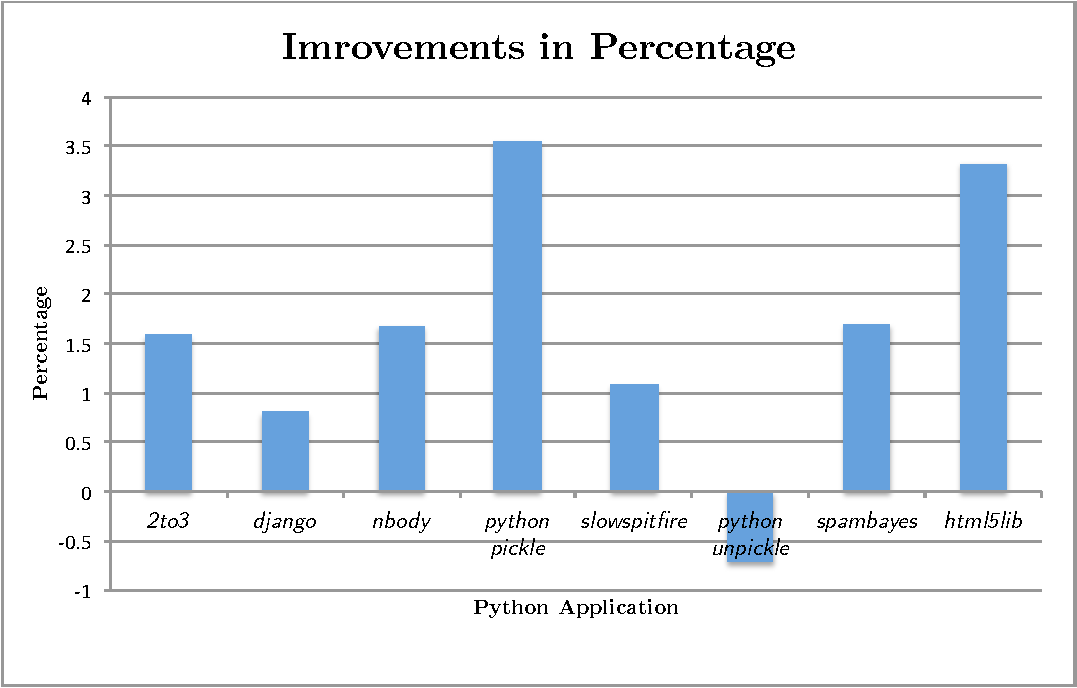
\includegraphics[width=12cm]{appsbench.pdf}
  \caption{Prcentage of overall improvements in some real-world Python applications. Nearly none of the applications performed worse. Python Pickle and html5lib faster around \%3 to \%4. }
\end{figure}

\begin{figure}[H]
  \centering
  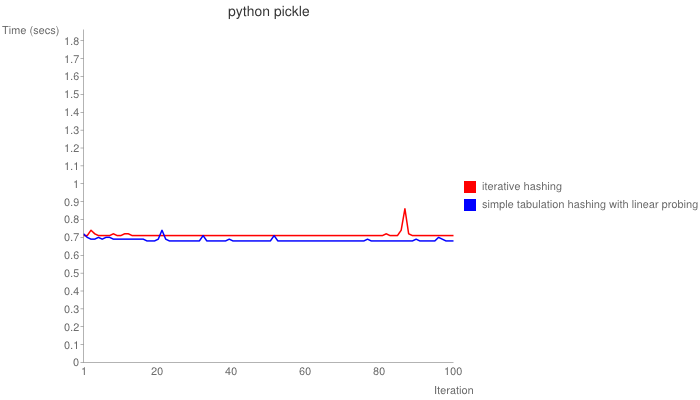
\includegraphics[width=12cm]{slowpickle.png}
  \caption{Python Pickle module benchmark. Minimum Iteration: changed from 0.705s to 0.681s: 1.04 times faster. Average iteration: changed from 0.710s to 0.686s: 1.04 times faster. Standard deviation of new implementation 2.0383 times smaller}
\end{figure}

% \begin{figure}[H]
%   \centering
%   \includegraphics[width=160mm]{lr-10.png}
%   \caption{}
% \end{figure}

% \begin{figure}[H]
%   \centering
%   \includegraphics[width=160mm]{lr-10.png}
%   \caption{}
% \end{figure}

In a couple of the programs such as pure Python Pickle (an object serialization library) and html5lib (specification parser library) we calculated an improvement of \%3 to \%4. In other cases we did not calculate an speedup but at the same time we did not find any real-world case which the new implementation performs significantly slower. These results were consistent with the previous results of PyBench that showed about \%4.5 improvement.
 
\section{Conclusion and future work}
Throughout the course of our work we came to the following conclusions:
\begin{enumerate}
\item Hardware specific performance issues dominate at small scales: When you are attempting to work on a process that runs as fast as a hash table lookup or insertion already does, there is little room for error.  Improving hash performance with simple tabulation is not an easy task simply because any change you make will probably end up making the hash table run slower.  That said:

\item Simple tabulation yields slightly faster and more consistent performance: With a careful implementation simple tabulation can yield increased hash performance on linear probing work loads. Simple tabulation definitely leads to shorter chain lengths, however, those shorter chain lengths don’t always justify the performance cost.

\item Memory latency presents serious but workable issues.  Doing a look up in the simple-tabulation table \emph{requires} a random memory access, exactly what we were trying to avoid. With careful memory management we can maintain good performance, but a solution requires careful thought about cache sizes and special purpose compiler directives.

\end{enumerate}

In terms of future work, we have 2 avenues of attack. First, we could use different dictionaries for different purposes. Many of the python dictionaries are small, and their keysets never change. No one is adding a new built-in function in the near future. 
Improve performance bottlenecks illustrated by benchmarks

\end{document}

